\documentclass{article}
\usepackage[margin=0.5in]{geometry}
\usepackage[utf8]{inputenc}
\usepackage{graphicx}
\usepackage{hyperref}
\usepackage{color}
\usepackage{amsmath,amssymb}
\usepackage{algorithm}
\usepackage{algorithmic}

\title{CMPSCI 383 Homework 2}
\author{\textbf{YOUR NAME HERE}}
\date{Assigned: Feb 21 2018; Due: March 5 2018 @ 11:59 PM EST}

\begin{document}

\maketitle

\begin{abstract}
    To submit this assignment, upload a pdf to Gradescope containing your responses to the written response questions below. You are required to use \LaTeX~for your write up. We suggest using sharelatex.com or overleaf.com, since they do not require you to install anything on your computer. When submitting your answers use the template \LaTeX~code provided and put your answers below the question they are answering. Do not forget to put your name on the top of the pdf. To submit the coding portion of the assignment upload your \texttt{my\_nqueens.py} file to the Gradescope programming assignment. Do not change function definitions or return types unless otherwise specified. Your work for all parts of this assignment must be your own (do not collaborate with other students in any way when completing this assignment). 
\end{abstract}

\section{N-Queens problem (60 pts)}
In class, we discussed various ways to tackle the classic N-Queens problem. In this section, you will first manually go over the hill climbing solution for this problem and then implement different solutions to the problem in python. 

\subsection{Hill climbing (20 pts)}
Given below is a random placement of four queens on a $4\times 4$ chess board. We will use the representation from class, where the board is represented by one number per column, denoting which row the queen is in. 

Find the next two moves for the board using hill climbing with the number of attacking pairs heuristic. As your answer to this question, provide the new board configurations represented as a list where the index represents the column and the value represents the row where the queen is present in that row. For reference, the representation of the initial board configuration is given.

\begin{figure}[h]
\centering
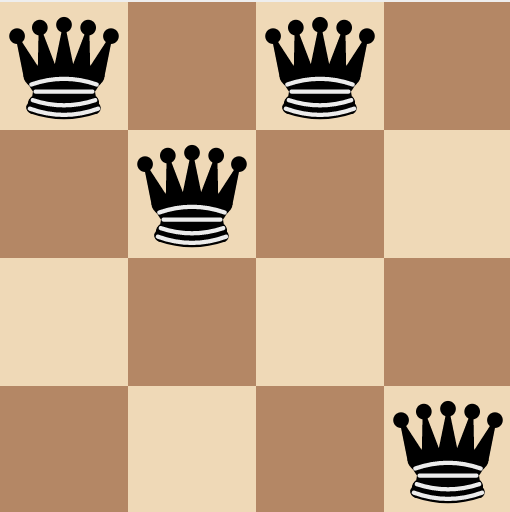
\includegraphics[width=5cm]{chess_board.png}
% * <subendhu.iitm@gmail.com> 2018-02-13T00:11:35.651Z:
%
% ^.
% * <subendhu.iitm@gmail.com> 2018-02-13T00:11:32.419Z:
%
% ^.
\caption{Initial configuration: [3,2,3,0]}
\end{figure}

\noindent \textbf{Answer:}
%Your response here

\subsection{Implementation (40 points) }
You will implement two different solutions to the N-Queens problem here using Python 3.6 using the anaconda distribution. Information about setting up the environment is given in the previous assignment. 

\subsubsection{Hill Climbing (20 points)}
Start from the template code in \texttt{my\_nqueens.py} and fill in the code for the required functions. Your program will take $n$ as an input and return the N-Queens solution for an $n\times n$ board. The solution should represented as a list of row indices as described in 1.1. You will use the hill climbing method here with the number of attacking pairs heuristic.

\subsubsection{Simulated Annealing (20 points)}
Start from the template code in \texttt{my\_nqueens.py} and fill in the code for the required functions. Your program will take $n$ as an input and return the N-Queens solution for an $n\times n$ board. The solution should be represented as a list of row indices as described in 1.1. You will use the simulated annealing method here with the number of attacking pairs heuristic. The temperature and annealing rate will be implemented as parameters to the annealing method.
\\ \\ 
Note that a solution might not always be found with a given starting board configuration using both these methods. You will therefore need keep track of whether a solution has been found in each run. 

\section{Genetic Algorithm for Sudoku (20 pts)}
In class, we looked at genetic algorithms that are designed to evolve candidate solutions into better solutions by combining them. Think about how you can apply this to solving the sudoku puzzle.

In your own words, describe how you would formulate the Sudoku puzzle as a GP search problem. Your answer should at least include information about the representation of the state as a string, the selection (fitness function), the mutation, and the cross-over methods you would use. 

\noindent \textbf{Answer:}
%Your response here

\section{Constraint Satisfaction Problems (20 pts)}
Read chapter 6 from the textbook about constraint satisfaction problems until section 6.3. Do exercise questions 6.1 and 6.2.
\noindent \textbf{Answer:}
%Your response here

\end{document}
